\documentclass[letterpaper,landscape,english,9pt]{report}
\usepackage[landscape,margin=0.5cm]{geometry}

\usepackage{fixltx2e} % LaTeX patches, \textsubscript
\usepackage{cmap} % fix search and cut-and-paste in PDF
\usepackage[T1]{fontenc}
\usepackage[utf8]{inputenc}
\usepackage{ifthen}
\usepackage{babel}
\usepackage{color}
\usepackage{float} % float configuration
\floatplacement{figure}{H} % place figures here definitely


\usepackage{multicol}
%\setlength{\columnseprule}{1pt} % for visible divider
\setlength{\columnsep}{1cm}

\usepackage{graphicx}
\graphicspath{
 {../pics/}
}

%%% Custom LaTeX preamble
% PDF Standard Fonts
\usepackage{mathptmx} % Times
\usepackage[scaled=.90]{helvet}
\usepackage{courier}

\usepackage{flowfram}
%\usepackage{booktabs}           % for rules in tables
\usepackage{tabularx}           % for column-width tables
\usepackage[table]{xcolor}      % color control

%\usepackage[colorlinks]{hyperref}

\usepackage{enumitem}           % useful for control of listings
\usepackage[compact,raggedright]{titlesec}
\usepackage{comment}

\newcommand{\epigraph}[3]{\textit{#1}\linebreak \vspace{-1.5em} \begin{flushright}\hspace{5em}\ --\ #2\linebreak\small{#3} \end{flushright}}

\pagestyle{empty}
\parindent=0pt

% Attempts to change bg color of *section headings
%\definecolor{secbgcol}{rgb}{0.9, 0.85, 0.85}
%\titleformat{\section}
%{\color{red}\normalfont\Large\bfseries}{\ndsection}{1em}{}
%\titleformat{\subsection}
%{\color{red}\normalfont\large\bfseries}{\begin{flushright}\hfill\thesubsection
%  \end{flushright}}{1em}{}
%
%\usepackage{pstricks}

% To create tables within multicols
\makeatletter
\newenvironment{ndtable}
  {\def\@captype{table}}
  {}


\newcommand{\ndheading}[3]{%
\vspace{0.5em}
\begin{ndtable}%
\rowcolors[\hline]{1}{#2}{} \arrayrulecolor{#3}
\begin{tabularx}{\columnwidth}{>{\centering\arraybackslash}X}\vspace{-.5em}\normalfont\large\bfseries
  #1\vspace{0.05em}\\\end{tabularx}
\end{ndtable}
\vspace{-.5em}
}

\definecolor{secfgcol}{RGB}{102, 153, 0}
\definecolor{secbgcol}{RGB}{216, 255, 137}
\definecolor{projfgcol}{RGB}{6,   83, 215}
\definecolor{projbgcol}{RGB}{255, 255, 205}

%\definecolor{secfgcol}{RGB}{6, 83, 215}
%\definecolor{secbgcol}{RGB}{241, 248, 255}
%\definecolor{projfgcol}{RGB}{6,   83, 215}
%\definecolor{projbgcol}{RGB}{241, 248, 255}

\newcommand{\ndsection}[1]{\ndheading{#1}{secbgcol}{secfgcol}}
\newcommand{\ndsubsection}[1]{\ndheading{#1}{secbgcol}{secfgcol}}

%\newcommand{\ndproject}[2]{\ndheading{\noindent#1\newline{\small\url{#2}}}{secbgcol}{secfgcol}}

\newcolumntype{V}{>{\arraybackslash} m{.2\linewidth} }
\newcolumntype{C}{>{\arraybackslash} m{.72\linewidth} }
\newcommand{\ndproject}[6]{%
\vspace{0.5em}
\begin{ndtable}%
\rowcolors[]{1}{projbgcol}{} \arrayrulecolor{projbgcol}
\begin{tabularx}{\columnwidth}{CV}\vspace{-.5em}\normalfont\large\bfseries
 #1 \newline {\small\url{#2}} &
 \vspace{#5}\hspace{#6}\includegraphics[width=#4\columnwidth]{../pics/#3}\vspace{-0.5em}\end{tabularx}
\end{ndtable}
\vspace{-.5em}
}

\newcommand{\ndcite}[1]{{\small #1}}
%%% User specified packages and stylesheets

%%% Fallback definitions for Docutils-specific commands

% admonition (specially marked topic)
\providecommand{\DUadmonition}[2][class-arg]{%
  % try \DUadmonition#1{#2}:
  \ifcsname DUadmonition#1\endcsname%
    \csname DUadmonition#1\endcsname{#2}%
  \else
    \begin{center}
      \fbox{\parbox{0.9\textwidth}{#2}}
    \end{center}
  \fi
}

% title for topics, admonitions and sidebar
\providecommand*{\DUtitle}[2][class-arg]{%
  % call \DUtitle#1{#2} if it exists:
  \ifcsname DUtitle#1\endcsname%
    \csname DUtitle#1\endcsname{#2}%
  \else
    \smallskip\noindent\textbf{#2}\smallskip%
  \fi
}

% hyperlinks:
\ifthenelse{\isundefined{\hypersetup}}{
  \usepackage[unicode,colorlinks=true,linkcolor=blue,urlcolor=blue]{hyperref}
  \urlstyle{same} % normal text font (alternatives: tt, rm, sf)
}{}

%%% Local Variables:
%%% mode: latex
%%% TeX-master: t
%%% TeX-PDF-mode: t
%%% End:


\hypersetup{
  pdftitle={Python in Electrophysiology},
}

%%% Body
\begin{document}

\begin{multicols}{3}    % 3 columns

% Document title
%\section*{
\begin{center}\Large \textbf{Python in Electrophysiology}\end{center}
%}
%\label{python-in-neuroimaging}

\begin{center}
\noindent
%% yoh: what logo?  worse comes to worse we could reuse snakebrain in
%%      different colorscheme ;)
\includegraphics[width=0.5\columnwidth]{snakebrain}
%\includegraphics[width=0.5\columnwidth]{openlogo-vsop}

Find the community @ \url{http://http://neuralensemble.org}

%% yoh: or what should be(come) the canonical location?
%%      or should we (you) come up with one?

% \hrule
\end{center}
\vspace{0em}


%___________________________________________________________________________
%% yoh: what sections do you foresee?  Below see my blunt dump of ideas
%%      or may be there should be no sections at all?

\ndsection{Data I/O}

%___________________________________________________________________________

% Your logo placed under ../pics called as <project>_logo.svg
% .svg is preferable, otherwise some other vector (.pdf) or even
% raster (.png) would suffice
\ndproject{XXX}{http://example.org}{opensesame_logo.pdf}{.2}{-0.25em}{0em}

%\begin{figure}
%
\includegraphics[width=0.3\columnwidth]{../pics/psychopy_logo.pdf}
%\end{figure}

Brief description.
\begin{itemize}[nolistsep,topsep=0em,leftmargin=1pc]
\item The most interesting
\item and
\item methodology oriented
\item features
\item ideally with limited selection of citations
\end{itemize}
% Your favorite screenshot placed under ../pics/
% named as <project>_screenshot.png (optional numbers in suffixes if
% you have multiple to choose from)
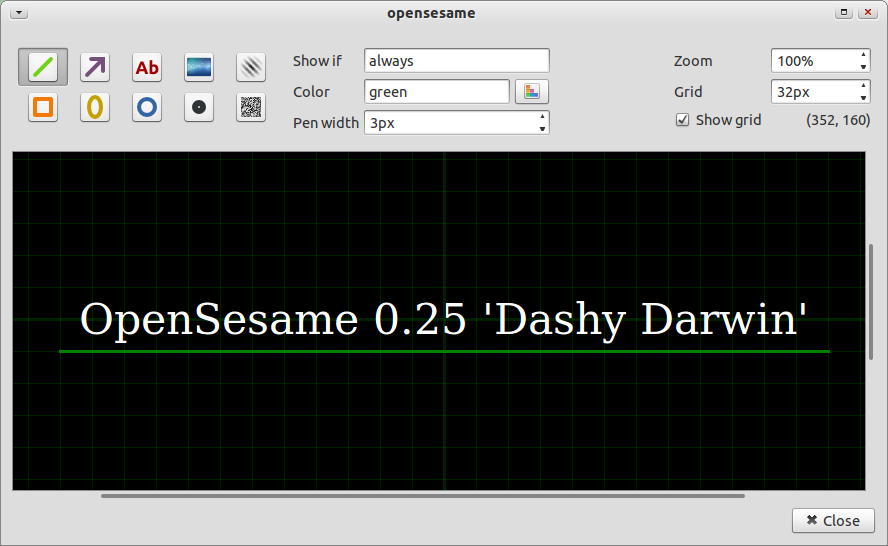
\includegraphics[width=\columnwidth]{opensesame_screenshot1.png}
% Selected set of citations, Here is an example:
\ndcite{D. Geffroy, D. Rivière, I. Denghien, N. Souedet,
  S. Laguitton, and Y. Cointepas. BrainVISA: a complete software
  platform for neuroimaging.  In Python in Neuroscience workshop,
  Paris, Aug. 2011.}


\ndproject{Neuroshare Tools}{http://g-node.org/neuroshare-tools}{blank.png}{.2}{-0.25em}{0em}

Load neuroshare compatible datafiles in Python.

\begin{itemize}[nolistsep,topsep=0em,leftmargin=1pc]
\item Access neuroshare compatible files directly from Python
\item Automatically detects file types and loads the corresponding neuroshare libraries
\item Use 32-bit MS Windows libraries under Linux \& Mac OS X with nsWineProxy 
\item High-level pythonic API that hides the details of the underlying C library
\item Support for Linux and Mac OS X
\end{itemize}


\ndproject{ns2hdf}{https://github.com/G-Node/ns2hdf}{blank.png}{.2}{-0.25em}{0em}

Converts any data-file that is supported by neuroshare to the HDF5 format.

%___________________________________________________________________________
\ndsection{Metadata Handling}%

\ndproject{odML libraries \& Editor}{http://www.g-node.org/odml/}{odml_logo.png}{.2}{-0.25em}{0em}

Use the {open metadata Markup Language} to annotate data with information about the stimulus, data acquisition, and experimental conditions.

\begin{itemize}[nolistsep,topsep=0em,leftmargin=1pc]
\item Developer friendly libraries for Python \& Java
\item Fully functional editor for Linux, Windows \& MacOS X
\item Support for the latest odML specification
\end{itemize}

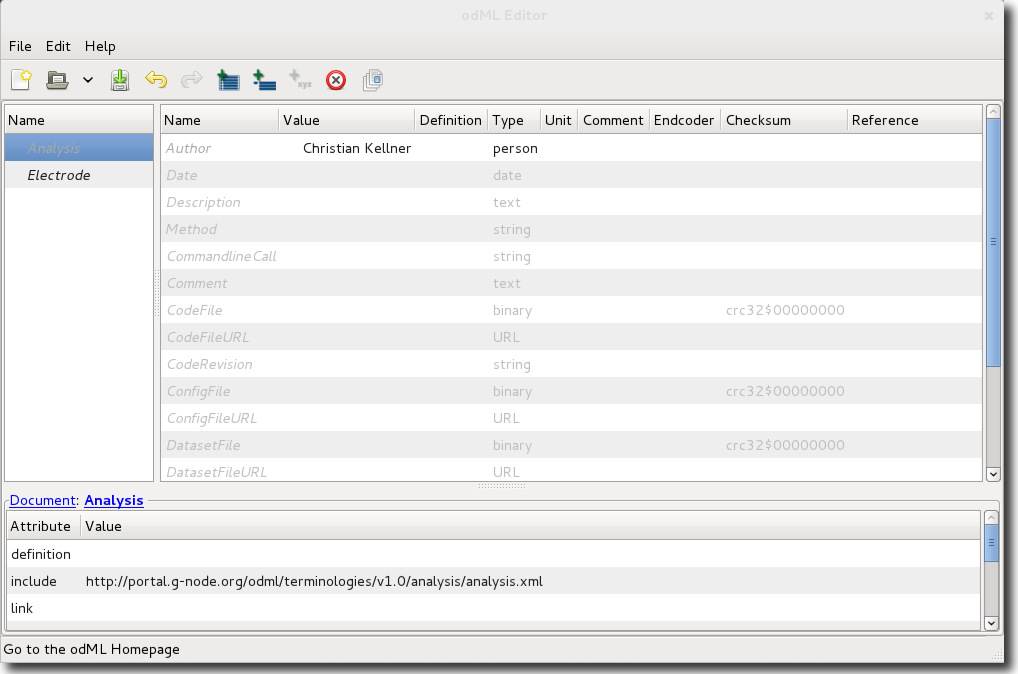
\includegraphics[width=\columnwidth]{odml_editor_screenshot.png}

\ndcite{J. Grewe, T. Wachtler and J. Benda. A bottom-up approach to data annotation in neurophysiology. In Front. Neuroinform. 5:16,
  2011. doi: 10.3389/fninf.2011.00016}
\ndsection{Data Archiving}
\ndsection{Experimentation Control}
\ndsection{Analysis}%

%________________________Stimfit____________________________________________

% Your logo placed under ../pics called as <project>_logo.svg
% .svg is preferable, otherwise some other vector (.pdf) or even
% raster (.png) would suffice
\ndproject{Stimfit}{http://www.stimfit.org}{stimfit_logo.png}{.2}{-0.25em}{0em}

%\begin{figure}
%
\includegraphics[width=0.3\columnwidth]{../pics/psychopy_logo.pdf}
%\end{figure}

Visualise and quantify electrophysiological data.
\begin{itemize}[nolistsep,topsep=0em,leftmargin=1pc]
\item With a focus on patch-clamp recordings
\item Supports most standard patch-clamp file types
\item Embedded Python shell
\item Measure action potential, EPSC and EPSP kinetics
\item Extract spontaneous and evoked events
\item Successfully used in many publications for >\,5 years
\end{itemize}
% Your favorite screenshot placed under ../pics/
% named as <project>_screenshot.png (optional numbers in suffixes if
% you have multiple to choose from)
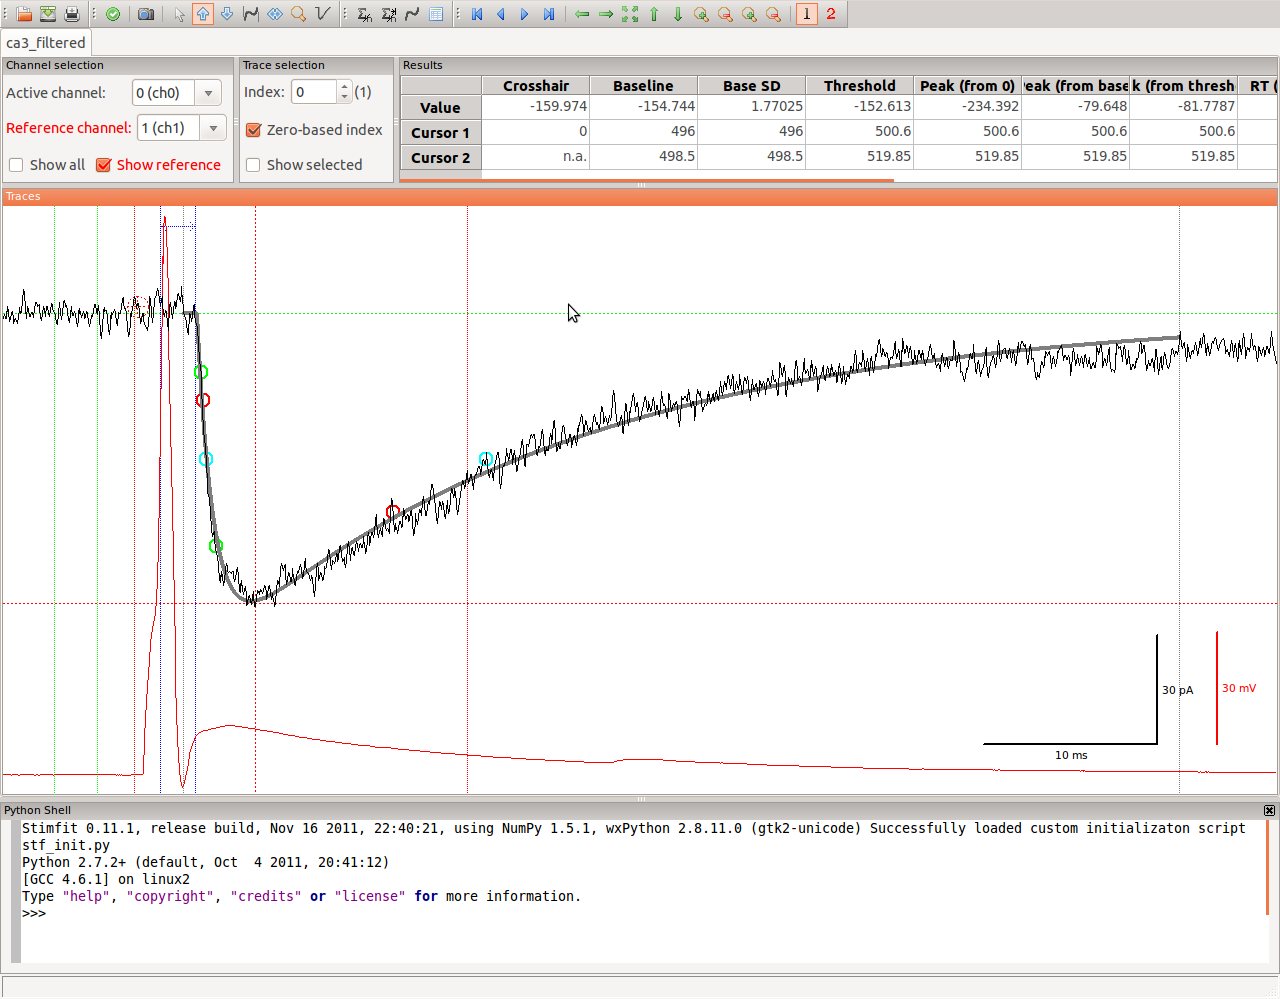
\includegraphics[width=\columnwidth]{stimfit_screenshot.png}
% Selected set of citations, Here is an example:
% Working on a manuscript right now ;-)

%___________________________________________________________________________

\ndsection{Closed-loop Frameworks}%

\end{multicols}
\end{document}

%%% Local Variables:
%%% mode: latex
%%% TeX-master: t
%%% TeX-PDF-mode: t
%%% whizzy-viewers: (("-pdf" "okular") ("-dvi" "xdvi") ("-ps" "gv"))
%%% End:
